\documentclass[tikz,border=2pt]{standalone}
\usepackage{tikz}
\usepackage{pgfplots}
\usetikzlibrary{intersections}
\usetikzlibrary{positioning}
\usetikzlibrary{backgrounds}
\usetikzlibrary{shapes.geometric}
\usetikzlibrary{shapes.arrows}
\definecolor{redd}{RGB}{255,0,0}
\definecolor{bluee}{RGB}{68,114,196}
\definecolor{greenn}{RGB}{0,176,80}

\begin{document}
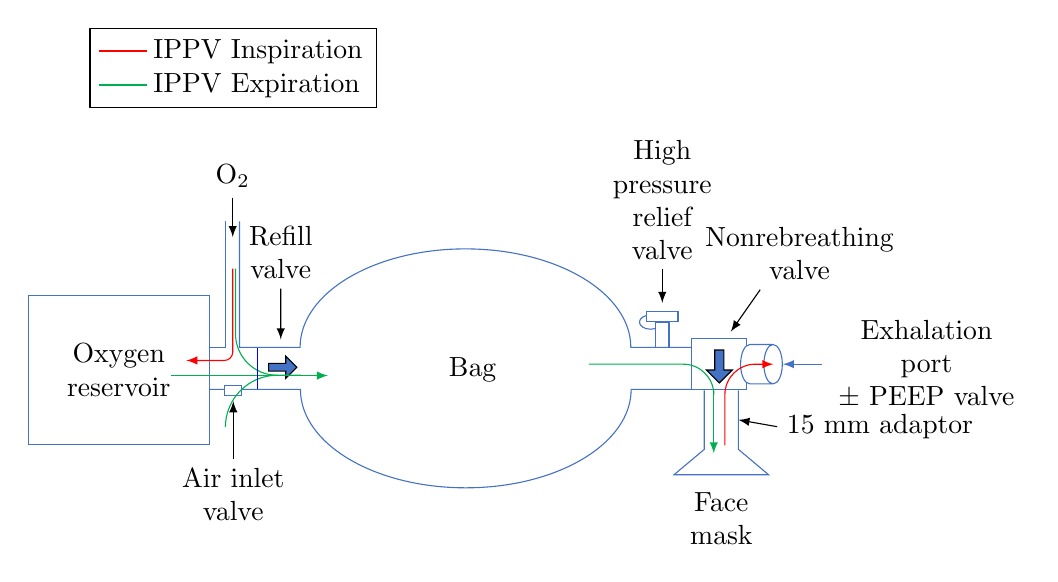
\begin{tikzpicture}
\node[]at(-0.5,0.21){Bag};
\node[draw=bluee,rectangle,anchor=south west,
minimum width=23mm, 
text width=20mm,align=center,
minimum height=19mm](B1)at(-6.15,-0.75){Oxygen reservoir};

\draw[bluee](B1.14)--++(0.2,0)--++(0,1.6)coordinate(O2);
\draw[bluee]([xshift=5]O2)--++(0,-1.6)--++(0.77,0)
arc(180:0:2.1 and 1.25)--++(0.9,0)coordinate(KG);

\draw[bluee](B1.348)--++(1.15,0)coordinate(SRE)
arc(-180:0:2.1 and 1.25)--++(0.9,0)coordinate(KD);

\node[draw=bluee,rectangle,anchor=south west,
minimum width=2.2mm, inner sep=0pt,
fill=white,
minimum height=1.2mm](B2)at([xshift=1.8mm,yshift=-0.8mm]B1.348){};

\draw[latex-,black,shorten <=2pt](B2.south)--++(0,-0.8)
node[black,below,text width=15mm,align=center]{Air inlet valve};

\node[single arrow,  draw=black,scale=0.6,
fill=bluee,minimum width=1ex, minimum height=1.2ex, 
single arrow head extend=1ex,
inner sep=0pt
](DA)at ([xshift=9mm,yshift=1pt]B1.east){\vphantom{a}\hspace*{5mm}};
\draw[shorten <=-5mm,-latex,greenn]([yshift=-2pt]B1.east)--++(1.5,0)coordinate(VA);
\draw[greenn]([yshift=-4mm,xshift=-1mm]B2.south)arc(180:90:0.66)coordinate(IS);

\draw[-latex,black]([xshift=0.9mm,yshift=3mm]O2)node[black,above]{O$_2$}
--++(0,-0.5)coordinate(VAA);

\draw[-latex,redd,shorten <=4mm,shorten >=-3mm](VAA){[rounded corners=3]|-(B1.6)};

\draw[greenn,shorten <=4mm,shorten >=-3mm]([xshift=1pt]VAA){[rounded corners=15]|-(IS)};

\draw[latex-,black,shorten <=3mm](DA)--++(0,1)
node[above,text width=15mm,align=center,black]{Refill \\ valve};

\draw[blue]([xshift=6mm]B1.348)--++(0,0.53);

\node[draw=bluee,rectangle,anchor=center,
minimum width=7mm, inner sep=0pt,
fill=white,
minimum height=6.5mm](BD1)at([xshift=2.2mm,yshift=3.2mm]KD){};

 \node (a) [cylinder, shape border rotate=0, anchor=east,fill=white,
  draw=bluee, minimum height=5.3mm, minimum width=5.0mm] 
  (CIL)at ([xshift=4.5mm]BD1.east){};
  
  \draw[bluee](BD1.240)--++(0,-0.75)--++
  (220:0.5)--coordinate(DNO)++(1.2,0)--++(140:0.5)--coordinate(PET)++(0,0.75);
  
  \draw[latex-,black](PET)--++(-10:0.5)node[black,right]{15 mm adaptor};
  \node[below=1mm of DNO,text width=12mm,align=center]{Face mask};
  
  \draw[latex-,bluee](CIL.east)--++(0.5,0)
  node[black,right,text width=24mm,align=center]{Exhalation port \\ $\pm$ PEEP valve};
  
  \draw[latex-,black,shorten <=1mm](BD1.75)--++(55:0.75)
    node[xshift=5mm,black,above,text width=27mm,align=center]{Nonrebreathing \\ valve};
 
 \node[single arrow,  draw=black,scale=0.7,
fill=bluee,minimum width=1ex, minimum height=1.2ex, 
single arrow head extend=1ex,rotate=270,
inner sep=0pt
](DA2)at (BD1){\vphantom{a}\hspace*{5mm}};


\draw[greenn,shorten <=13mm,shorten >=0mm]
(BD1.west){[rounded corners=11]-|(BD1.258)};
\draw[greenn,-latex](BD1.258)--++(270:0.8);

\draw[redd,shorten >=7mm,shorten <=2mm,]
(BD1.east){[rounded corners=11]-|(BD1.282)};
\draw[redd,-latex]([xshift=2pt]BD1.east)--++(0:0.26);

%Pressure
\begin{scope}[on background layer]
\node[draw=bluee,shape=ellipse,minimum height=1.8mm,minimum width=2.8mm,
inner sep=1pt] (CI2)
at([xshift=-6.5mm,yshift=3.2mm]KG){};
\node[draw=bluee,rectangle,anchor=south,
minimum width=1.7mm, inner sep=0pt,
fill=white,
minimum height=3.2mm](PRE)at([xshift=-5.0mm,yshift=-0.2pt]KG){};

\node[draw=bluee,rectangle,anchor=south,
minimum width=4.0mm, inner sep=0pt,
fill=white,
minimum height=1.3mm](PRE2)at([xshift=0mm,yshift=-0.2pt]PRE.north){};

\draw[latex-,black,shorten <=1mm](PRE2)--++(90:0.6)
    node[black,above,text width=27mm,align=center]{High\\pressure\\relief\\ valve};
\end{scope}

    \begin{axis}[
    hide axis,
    xmin=10,
    xmax=50,
    ymin=0,
    ymax=0.1,
    legend style={legend cell align=left, at={(-0.25,0.8)}}
    ]
    \addlegendimage{redd, thick}
    \addlegendentry{IPPV Inspiration};
    \addlegendimage{greenn, thick}:
    \addlegendentry{IPPV Expiration}:
    \end{axis}

\end{tikzpicture}
\end{document}
